\documentclass[conference]{IEEEtran}
\usepackage{times}

% numbers option provides compact numerical references in the text. 
\usepackage[numbers]{natbib}
\usepackage{multicol}
\usepackage[bookmarks=true]{hyperref}

\pdfinfo{
   /Author (author)
   /Title  (title)
   /CreationDate (D:20101201120000)
   /Subject (Robots)
   /Keywords (Robots)
}

\usepackage{microtype}
\usepackage{amsmath,amssymb}
\usepackage{paralist}
\usepackage{mdframed}
\usepackage{xcolor}
\usepackage{tikz}
\usepackage{amsthm}
\usepackage{amssymb}
\usepackage{nicefrac}
\usepackage{amsthm}
\usepackage{colonequals}
\newtheorem{theorem}{Theorem}
\newtheorem{proposition}{Proposition}
\theoremstyle{remark}
\newtheorem{remark}{Remark}
\newtheorem{example}{Example}
\newtheorem{definition}{Definition}


\usetikzlibrary{patterns,arrows,backgrounds,calc,shapes,shadows,decorations.pathmorphing,decorations.pathreplacing,automata,shapes.multipart,positioning,shapes.geometric,fit,circuits,trees,shapes.gates.logic.US,fit,decorations.markings}

\tikzset{sstate/.style={circle, draw=black, inner sep=1pt,minimum height=6mm}}
\tikzset{astate/.style={diamond, draw=black, inner sep=1pt}}
\tikzset{tstate/.style={rectangle, draw=black, inner sep=1pt, minimum height=5mm}}
\tikzset{actnode/.style={fill=black, inner sep=1pt}}
\tikzset{elab/.style={auto,font={\fontsize{9pt}{12}\selectfont}}}

\makeatletter
\let\MYcaption\@makecaption
\makeatother

\usepackage[font=footnotesize]{subcaption}

\makeatletter
\let\@makecaption\MYcaption
\makeatother

\newcommand{\NN}{\mathbb{N}}
\newcommand{\mc}{\mathcal{D}}
\newcommand{\sg}{\mathcal{G}}
\renewcommand{\path}{\xi}
\newcommand{\eventually}[1]{\lozenge^{\leq #1}}
\newcommand{\sched}{\sigma}
\newcommand{\Sched}{\Sigma}
\newcommand{\pol}{\sched}
\newcommand{\Distr}{\ensuremath{\textsl{Distr}}}
\newcommand{\act}{\alpha}
\newcommand{\altact}{\beta}
\newcommand{\Act}{A}
\newcommand{\scp}{p}
\newcommand{\scthreshold}{\mathbf{p}}
\newcommand{\target}{s_{\top}} 
\newcommand{\sink}{s_{\bot}}
\newcommand{\rndp}{h}
\newcommand{\randomness}{\mathbf{h}}
\newcommand{\last}[1]{\mathsf{last}({#1})}
\newcommand{\pOneSched}{\mathbf{ego}}
\newcommand{\POneScheds}{\Sigma_\pOne}
\newcommand{\PTwoScheds}{\Sigma_\pTwo}
\newcommand{\pTwoSched}{\mathbf{env}}
\newcommand{\rat}{\lambda}
\newcommand{\pOne}{\mathsf{ego}}
\newcommand{\pTwo}{\mathsf{env}}
\newcommand{\horizon}{\tau}
\newcommand{\solutions}{\mathbb{S}}
\newcommand{\EnAct}{\Act}
\newcommand{\solfuncp}{f_\mathbb{S}}
\newcommand{\scopt}{\scp^{*}}
\newcommand{\rndopt}{\rndp^{*}}
\newcommand{\pareto}[1]{\mathcal{F}_{#1}}
\newcommand{\smoothmax}[1]{\mathsf{smax}(#1)}
\newcommand{\indicator}[1]{[#1]}
\newcommand{\Succ}{\mathsf{Succ}}
\newcommand{\supp}{\mathsf{supp}}

\newcommand{\scmin}{\scp^{-}}
\newcommand{\rndmin}{\rndp^{-}}
\newcommand{\pathslbl}{\Xi}
\newcommand{\Paths}[2][]{\pathslbl^{#2}_{#1}}
\newcommand{\POnePaths}[2][]{{\pathslbl^{#2}_{#1}}/_{\downarrow_{1}}}
\newcommand{\PTwoPaths}[2][]{{\pathslbl^{#2}_{#1}}/_{\downarrow_{2}}}
\newcommand{\PiPaths}[2][]{{\pathslbl^{#2}_{#1}}/_{\downarrow_{i}}}
\newcommand{\unrolled}[2]{\textsf{Tree}(#1,#2)}
\newcommand{\induced}[2]{#1[#2]}
\newcommand{\causalprob}[2]{\Pr(#1\mid\mid#2)}
\newcommand{\expOver}[2]{\mathbb{E}_{#1}[#2]}



\setlength\marginparwidth{110pt}
\newcommand{\colorpar}[3]{\colorbox{#1}{\parbox{#2}{#3}}}
\newcommand{\marginremark}[3]{\marginpar{\colorpar{#2}{\linewidth}{\color{#1}#3}}}
\newcommand{\commentside}[2]{\marginpar{\color{#1}\tiny#2}}
\newcommand{\TODO}[1]{\commentside{teal}{\textsc{Todo:} #1}}
\newcommand{\REMARK}[1]{\commentside{teal}{\textsc{Remark:} #1}}\newcommand{\sj}[1]{\marginremark{black}{red!10!white}{\scriptsize{[SJ]~ #1}}}
\newcommand{\mvc}[1]{\marginremark{black}{gray!10!white}{\scriptsize{[MVC]~ #1}}}


%\institute{University of California, Berkeley, CA, USA}


\begin{document}

% paper title
\title{Entropy-Guided Control Improvisation}

% You will get a Paper-ID when submitting a pdf file to the conference system
\author{Author Names Omitted for Anonymous Review. Paper-ID [add your ID here]}

%\author{\authorblockN{Michael Shell}
%\authorblockA{School of Electrical and\\Computer Engineering\\
%Georgia Institute of Technology\\
%Atlanta, Georgia 30332--0250\\
%Email: mshell@ece.gatech.edu}
%\and
%\authorblockN{Homer Simpson}
%\authorblockA{Twentieth Century Fox\\
%Springfield, USA\\
%Email: homer@thesimpsons.com}
%\and
%\authorblockN{James Kirk\\ and Montgomery Scott}
%\authorblockA{Starfleet Academy\\
%San Francisco, California 96678-2391\\
%Telephone: (800) 555--1212\\
%Fax: (888) 555--1212}}


% avoiding spaces at the end of the author lines is not a problem with
% conference papers because we don't use \thanks or \IEEEmembership


% for over three affiliations, or if they all won't fit within the width
% of the page, use this alternative format:
% 
%\author{\authorblockN{Michael Shell\authorrefmark{1},
%Homer Simpson\authorrefmark{2},
%James Kirk\authorrefmark{3}, 
%Montgomery Scott\authorrefmark{3} and
%Eldon Tyrell\authorrefmark{4}}
%\authorblockA{\authorrefmark{1}School of Electrical and Computer Engineering\\
%Georgia Institute of Technology,
%Atlanta, Georgia 30332--0250\\ Email: mshell@ece.gatech.edu}
%\authorblockA{\authorrefmark{2}Twentieth Century Fox, Springfield, USA\\
%Email: homer@thesimpsons.com}
%\authorblockA{\authorrefmark{3}Starfleet Academy, San Francisco, California 96678-2391\\
%Telephone: (800) 555--1212, Fax: (888) 555--1212}
%\authorblockA{\authorrefmark{4}Tyrell Inc., 123 Replicant Street, Los Angeles, California 90210--4321}}


\maketitle

\begin{abstract}
Declarative constraints are a powerful tool to define high-level controllers. 
However, most algorithms that synthesise controllers from these constraints construct deterministic policies -- which limits robustness and unpredictability.  
Control improvisation aims to overcome these weaknesses. Key are three types of constraints: Hard constraints describe behavior that must occur, 
soft constraints describe behavior that typically occurs, and a randomization constraint ensures variance in the behavior. 
We provide the first control improvisation framework, based on causal entropy to describe randomization, that supports to adverserial and probabilistic environments. These features allow us to synthesise powerful robust policies that generate unpredictable behavior. 

\end{abstract}

\IEEEpeerreviewmaketitle

%\maketitle\sj{Daniel?}
%\begin{abstract}
%	Efficacious controller synthesis is a key ingredient in the design and analysis of complex systems. We study the design of controllers that have a high entropy, that is, whose behavior or nature is surprising. The synthesis of such controllers is key in domains like testing and security. 
%	In particular, our paper studies control improvisation and compares them with randomly sampling adequate policies. The only difference in obtained policies is in their notion of entropy, but the problems are significantly different.  We illustrate and contrast their merits and limitations. Furthermore, we provide algorithms that solve both control improvisation problems. Prominently, we solve the control improvisation problem for Markov decision processes by relating it to recent results from inference from demonstrations, and then extend this approach to stochastic games. We present a prototypical implementation that efficiently solves controller synthesis problems from the security and testing domain. 
%\end{abstract}
\section{Introduction}
% Declarative Constraints ar neat idea.
The use of declarative specifications, e.g. in the form of temporal logic formulas, has become a popular way to construct high-level robot controllers~\cite{DBLP:conf/iros/HorowitzWM14, DBLP:conf/rss/WongEK14, DBLP:conf/iros/HeLKV17, DBLP:conf/icra/FuATP16, DBLP:conf/icra/HeWKV19, DBLP:journals/arobots/MoarrefK20, DBLP:conf/icra/KantarosM0P20}.
% Synthesis closes the gap.
Given a user provided specification, \emph{synthesis} algorithms aim
to automatically create a control policy that ensures that the
specification is met, or explain why such a policy does not
exist. Together, synthesis and declarative specifications facilitate
quickly and intuitively solving a wide variety of control tasks.  For
example, consider a delivery drone operating in a workspace. One may
specify the drone should ``within 10 minutes, visit four locations (in any
order) \emph{and} avoid crashing.''. A synthesis tool may then create a
finite state controller which guarantees this specification is met,
under a particular world model.
% Declarative Synthesis need not produce variety.  
Importantly, while many controllers may conform to the
provided specification, many synthesis algorithms provide a
single, often deterministic, policy.  For instance, in our drone
example, a synthesized controller may generate only a single path
through the workspace.

% On the importance of being varied.
In some settings, such policies however are undesirable.  First, in
many tasks, the predictability (or bias) of the policy may be a
liability.  Examples include
patrolling~\cite{DBLP:journals/ior/AlpernMP11}, behavior prediction
and inference~\cite{DBLP:conf/cav/Vazquez-Chanlatte20}, and creating
controller harnesses for fuzz testing (see motivating
example). Second, synthesis algorithms work on \emph{idealized}
models, and thus any policy that overcommits to any given model quirk
may in practice yield poor performance. In such settings,
randomization is known to make policies more robust against worst-case
deviations~\cite{mceThesis, maxEntAnswer}. Unfortunately, classical 
synthesis methods result in policies that need not (and typically do
not) exhibit randomization.

% Propose CI and highlight new features.
To address these potential deficits, we advocate for the adoption of
the recently proposed control
improvisation~\cite{DBLP:conf/cav/FremontS18,DBLP:conf/fsttcs/FremontDSW15}
framework, in which one specifies a controller with three types of
declarative constraints. (i) \emph{Hard constraints} that, as in the
classical setting, must be satisfied, (ii) \emph{soft constraints} that
on most executions should hold, and (iii) \emph{randomization
constraints} that ensure that a synthesized policy does not overcommit to a particular action or behavior. 
The key challenge when solving control improvisation is that randomization and performance, in the form of soft constraints, constitute a natural trade-off.

Unfortunately, control improvisation has so far been limited to
nondeterministic domains where uncertainty is resolved
adversarially. This assumption is often too restrictive and leads
(together with the soft/hard constraints) to conservative policies or
common situations in which the synthesis algorithm cannot be employed
at all. To overcome this weakness, we develop a theory of control
improvisation in stochastic games which admit
arbitrary \emph{combinations} of nondeterministic and probabilistic
uncertainty, including unknown or imprecise transition
probabilities. 

Technically, we formulate our problem on \emph{simple stochastic
games}~\cite{DBLP:conf/dimacs/Condon90}, an extension of \emph{Markov decision processes} (MDPs) that divides states
between controllable states and uncontrollable (or adversarially
controlled) states. \emph{Soft constraints} are finite horizon
temporal properties with a threshold on the worst-case probability of
that the property holding by the end of the episode. \emph{Hard
constraints} are soft constraints to be satisfied with probability 1. In
contrast to other work on control improvisation, we adopt causal entropy as a natural means to formalize \emph{randomness
constraints}.  Causal entropy is a prominent notion in directed
information theory~\cite{DirectedInfoTheoery} that strongly correlates with robustness in the
(inverse) reinforcement learning setting~\cite{mceThesis,
maxEntAnswer}. We refer to this variant of control improvisation as
\emph{Entropic Reactive Control Improvisation} (ERCI) and show that ERCI
conservatively extends reactive control improvisation~\cite{DBLP:conf/cav/FremontS18} to stochastic
games. More precisely, entropy can
be used in the non-stochastic setting and yields results analogous to
reactive control improvisation. ERCI also extends  classical policy synthesis in stochastic games, i.e. synthesis in absence of randomness constraints as, e.g., implemented in PRISM-games~\cite{DBLP:journals/sttt/KwiatkowskaPW18}.


%We argue that soft constraints can naturally be considered as an
%optimization objective which one can trade-off for more randomization.
%Indeed, our method strongly relies on the computation of a
%Pareto-front that explores the trade-off between randomization and
%optimizing the soft constraint using the notion of rationality. This
%means that rather than asking the user to fix rather arbitrary
%threshold values for both types of constraints, we may visualize the
%trade-off between these two entities.
%
\mypara{Contributions}
In summary, this paper contributes ERCI, an algorithmic way to trade
performance and randomization in stochastic games. As we motivate in
the example below, games that combine both adversarial and
probabilistic behavior in an environment allows for modeling
flexibility, facilitate applicability to new domains. To support this
extension, the paper proposes and shows the benefits of formulating
randomization constraints with causal entropy.  Finally, this work
contributes the necessary technical machinery and a prototype 
implementation. Combined, our theoretical and empirical analysis
suggest that the ERCI framework contributes a tractable and flexible
modeling formalism.

\mypara{Overview} This paper is structured as follows. We begin with a
motivating example (Sec.~\ref{sec:motivating}). Then we provide
preliminaries and formalize the ERCI problem statement
(Sec.~\ref{sec:problem}). Next, we cast ERCI
as a multi-objective optimization problem and study properties of the
solution set (Sec.~\ref{sec:convex}). With this technical machinery developed,
Sec.~\ref{sec:mdps} re-frames existing literature on maximum causal
entropy inference and control to derive an algorithm for MDPs.  Then in Sec.~\ref{sec:sgs}, we provide an
algorithm for the general case of stochastic games. We conclude with
an empirical evaluation (Sec.~\ref{sec:empirical}) and a comparison
with related work, e.g., other control improvisation
formulations (Sec.~\ref{sec:related}). Proofs are attached in Sec.~\ref{sec:proofs}.



%%% Local Variables:
%%% mode: latex
%%% TeX-master: "main"
%%% End:

\section{Motivating Example}
\label{sec:motivating}
We consider high-level planning for drones. We consider a setting with a controllable drone $D$ and in presence of a secondary drone $E$. 
We partition the airspace into different zones. Four zones are marked as special points of interest (POIs).
One of the zones in a corner is a recharge station, where $D$ initially starts. $E$ starts in the opposite corner. We assume perfect observability.  
For safety, our plan must (\emph{hard constraint}) ensure that the two drones are never in the same zone. We are only interested in plans that visit the four POIs within a given time horizon (\emph{hard constraint}).
We should (\emph{soft constraint}) ensure that we do not run out of battery with high probability. 
Our aim is to create a plan such that the paths of $D$ within its environment are maximally unpredictable, i.e., we want to maximally randomize over the paths that satisfy the constraints. Due to the nature of the soft constraint, some of the paths that we include may violate this constraint. 

We discuss three different aspects of this setting.
Let us first start in absence of $E$. 
The main task here is to ensure power-aware scheduling, i.e., depending on the state of charge of the battery, we want to adapt our plan. Crucial in this is an adequate model of the battery. 
Both the battery quality itself and the power consumption are, however, uncertain. 
In particular, simply assuming that the battery is discharged with the average power consumption is unrealistic~\cite{DBLP:conf/cyphy/HermannsKN15}, and assuming that the battery is discharged with the maximal power consumption is too pessimistic. 
We use a model in which we discretize the battery charge, and in every time step the battery charge decrements by one step with some probability $p$. 
Overall, this yields a binomial distribution over the maximal steps until the battery is depleted.

Orthogonally, let us consider drone $E$. In the best case, drone $E$ is a delivery drone delivering packages along a fixed route. We can encode this route into the model. Compare Fig.~\ref{} without a drone $E$ and Fig.~\ref{} with drone $E$ flying the path marked in red. 

Orthogonally, as the drone $E$ is not controlled by us, we may want to make no assumptions on the behavior of $E$ and show that our plan for $D$ is robust for every possible behavior of $E$. 

We stress that this is different from assuming random behavior of $E$: We are interested in a policy that is good for any behavior of $E$, whereas assuming (uniform) random behavior for $E$ is good in expectation.
Such behavior may be overly pessimistic. 
In our example, we may have observed that $E$ delivers packets to the POIs, and thus some behavior is more likely. We may learn a model for this using inverse reinforecement learning. 
Clearly, we can plan much more liberally when we k

We can also mix this stochastic behavior with nondeterminism. For example, 

A natural criticism for stochastic models is the dependence on fixed probabilities. However, notice that we can combine adversarial choices and stochastic behavior such that we may model ranges of possible transition probabilities. More precisely, we support interval-valued transition probabilities. Consider the delivery-drone $E$. Rather than inferring a point-estimate from data, we may have inferred that the probability of turning around is in the interval $[p - \varepsilon, p + \varepsilon]$ for adequate values of $p$ and $\varepsilon$.  Furthermore the actual probability may even depend on aspects of the current state. 

Finally, the strength of the (entropy-guided) control improvisation framework is that we can combine all these aspects into a single computational model, which is very flexible. One aspect we want to highlight here is the implicit construction of a Pareto-curve that 






\begin{figure}
  \centering \scalebox{0.4}{
    \import{imgs/}{motivating_example.pdf_tex} }
  \caption{ Illustration of delivery drone testing example. The goal
    is to synthesize a policy for the bottom left (white circle) drone
    to test the controller of the top right (black square) drone. Ideally,
    the synthesized policy should be as randomized to avoid testing bias.\label{fig:motivating} }
\end{figure}

\begin{figure*}

\caption{Plans for different models of drone $E$}	
\end{figure*}

% Setup Testing Premise.
We consider a hypothetical scenario in which a regulatory agency
wishes to certify the safety and performance of a new delivery drone.
In order to do so, the agency may wish to run this new drone, call
$\droneEnv$, through a series of tests. For example, given a certain
delivery route, can $\droneEnv$ successfully deliver packages while
avoiding \emph{other} delivery drones. To do so, the agency decides to
synthesize a controller for another delivery drone, $\droneEgo$, and test if
$\droneEnv$ can be certified.

% Paint a picture.
Concretely, suppose we have high-level models (e.g. motion planners)
for $\droneEnv$ and $\droneEgo$, and suppose we can command
$\droneEnv$ to continuously visit four houses in our workspace. We
illustrate such a scenario in~Fig.~\ref{fig:motivating}, in which
$\droneEnv$ and $\droneEgo$ are shown as black square and white circle
drones respectively.  For this test scenario, the regulatory agency,
wishes to exam how $\droneEnv$ responds to delivering packages to the
red houses in the presence of $\droneEgo$. To test $\droneEnv$, the
agency wishes to have $\droneEgo$ also deliver packages while avoiding
$\droneEnv$.  Ideally, this $\droneEgo$'s policy should be as
un-biased as possible to exercise $\droneEnv$ on a variety of
scenarios, and ideally capture and sensor, software, or hardware
errors, e.g., a bug in a machine learned perception sensor.

% Frame as RCI.
With the ERCI framework, the agency may formalize the above scenario with the
following constraints on $\droneEgo$:
\begin{enumerate}
\item (\emph{hard constraint}) Ensure that the two drones \emph{never} collide.
\item (\emph{soft constraint}) With probability at least $.8$, visit all four houses within 10 minutes.
\item (\emph{randomness constraint}) Perform this task as unpredictability as possible.
\end{enumerate}
What then remains is to synthesize a controller given the constraints
\emph{and} the world model. At this point, it is worth examining more
closely how one models $\droneEnv$'s controller when synthesizing
$\droneEgo$. We illustrate by examining four models.

\mypara{Deterministic Model}
In the simplest case, the manufacture might guarantee that a
$\droneEgo$ will deliver packages on a fixed route. While tempting to
believe, such a route may be hard to a-priori compute and sensitive to
the exact details of the test workspace.

\mypara{Adversarial Model}
After testing $\droneEnv$, one might discover that it always visits
the houses in either clock-wise or counter-wise order, but seems to
switch direction non-deterministically.  As a first step, one might
model $\droneEnv$ as acting adversarially. Note however that such a
model is clearly too pessimistic -- there is no policy that satisfies
our constraints -- and frankly unrealistic within the context.
Furthermore, even if there existed a winning policy, such a pessimistic
model would result in an unnecessarily conservative (and thus predictable)
test controller, limiting its utility.

\mypara{Stochastic Model}
Next, after examining the data, one observes that $\droneEnv$ appears
to flip a biased coin whenever it reaches a house to decide whether or
not to turn around. The resulting Markov Decision Process may be
sufficiently correct to synthesize adequate improvisers without
being too pessimistic.

\mypara{Stochastic Games} However, a natural criticism for stochastic
models is the dependence on \emph{fixed} probabilities.  In our
example, we may have observed $\droneEnv$'s behavior and extracted
(point-)estimate probabilities, but these probabilities may still have
non-trivial error margins or could be sensitive to changes in the
workspace.  In absence of (enough or reliable) data, we can combine
adversarial choices and stochastic behavior such that we may model
ranges of possible transition probabilities.  More precisely, we
support interval-valued transition probabilities.  Consider the
delivery-drone $\droneEnv$. Rather than inferring a point-estimate
from data, we may have inferred that the probability of turning around
is in the interval $[p - \varepsilon, p + \varepsilon]$ for adequate
values of $p$ and $\varepsilon$.  Furthermore the actual probability
may even depend on aspects of the current state.

% Bring it all together.
\mypara{ERCI as a unifying framework}
The strength of the (entropy-guided) control improvisation framework
is that we can combine all these aspects into a single (flexible)
computational model. For example, we shall provide an algorithm that
can maximally randomize for all of the model discussed above. In the
coming sections, we shall formally define the ERCI problem, highlight
that there is an implicit trade-off between performance of the soft
constraint and unpredictability, and provide algorithms to solve ERCI
in Stochastic Games which admit arbitrarily combining adversarial and
probabilistic uncertainty.

% Pareto-curve that shows how randomization and performance yield a tradeoff. This means that rather than a-priori selecting threshold for entropy and the probability of not running out of battery, we obtain a variety op options and select the trade-off that is most satisfactory. Consider Fig.~\ref{}.


% We consider high-level planning for drones. We consider a setting with a controllable drone $D$ and in presence of a secondary drone $E$. 
% We partition the airspace into different zones. Four zones are marked as special points of interest (POIs).
% One of the zones in a corner is a recharge station, where $D$ initially starts. $E$ starts in the opposite corner. We assume perfect observability.  
% For safety, our plan must (\emph{hard constraint}) ensure that the two drones are never in the same zone. We are only interested in plans that visit the four POIs within a given time horizon (\emph{hard constraint}).
% We should (\emph{soft constraint}) ensure that we do not run out of battery with high probability. 
% Our aim is to create a plan such that the paths of $D$ within its environment are maximally unpredictable (random constraint), i.e., we want to maximally randomize over the paths that satisfy the constraints. Due to the nature of the soft constraint, some of the paths that we include may violate this constraint.  We apply our novel entropy-guided control improvisation. In the folllowing, we discuss different aspects of this setting.

% Let us first start in absence of $E$. 
% The main task here is to ensure power-aware scheduling, i.e., depending on the state of charge of the battery, we want to adapt our plan. Crucial in this is an adequate model of the battery. 
% Both the battery quality itself and the power consumption are, however, uncertain. 
% In particular, we may model that in every step deterministically the average power is consumed, but this plan will not be robust to any other behavior, and the plan is unrealistic~\cite{DBLP:conf/cyphy/HermannsKN15}. Typically, in synthesis, the other extreme is assumed (any amount of power can be drawn in every step). In this setting, this assumption leads the battery to be discharged with the maximal power consumption -- while this is clearly too pessimistic -- there is no policy that satisfies our constraints.
% We use a model in which we discretize the battery charge, and in every time step the battery charge decrements by one step with some probability $p$. 
% Overall, this yields a binomial distribution over the maximal steps until the battery is depleted.
% In Fig.~\ref{fig:motivating:batteries}, we show paths with a larger and smaller battery. As to be expected, the larger battery allows for more freedom in randomizing, as it is easier to meet the soft constraint.

% Orthogonally, let us consider drone $E$. 
% In the best case, drone $E$ is a delivery drone delivering packages along a fixed route. We can encode this route into the model. 
% Compare Fig.~\ref{} without a drone $E$ and Fig.~\ref{} with drone $E$ flying the path marked in red. 
% We can see how fewer paths meet the hard constraint, and thus, $D$ randomizes over fewer paths. 
% The plans in Fig.~\ref{} are not very robust: what if $E$ occasionally decided to return to its base (e.g., to recharge). More precisely, in Fig.~\ref{} we illustrate the policy for $D$ if we assume that $E$ flips a biased coin in every step in which it decided to turn around.
% We observe that this decreases the paths that satisfy the hard guarantee (not crashing) and indirectly also means that it becomes more likely that we deplete the battery due to evading $E$.
% Finally, rather than assuming some stochastic behavior where $E$ turns around, we may want to not make any assumption on under which circumstances or what probability $E$ turns. 
% The difference is more subtle: changing from randomization to adversarial behavior of $E$ does not change the set of paths that violate the hard constraint, $D$ will need to evade $E$ more often, yielding higher battery consumption. 
% More generally, the difference between assuming random behavior of $E$ and adversarial behavior is as follows: In the latter case, we are interested in a policy that is good for any behavior of $E$, that is, it is good in the worst-case, whereas assuming (uniform) random behavior for $E$ in expectation, but does not give guarantees on the worst-case. Generally, optimizing for the worst-case is overly pessimistic.


%%% Local Variables:
%%% mode: latex
%%% TeX-master: "main"
%%% End:

\section{Problem Statement}
\label{sec:problem}
This section formalizes the problem statement.  We start with some necessary definitions and notations.


\subsection{Stochastic Games}
An (2.5-player) \emph{stochastic game} (SG) is a tuple $\sg = \langle S, \iota, \Act, P \rangle$. The set of \emph{states} $S = S_1 \cup S_2$ is partitioned into a set $S_1$ of player-1 states and a set $S_2$ of player-2 states. $\iota \in S$ is the \emph{initial state}, $\Act = \Act_1 \cup \Act_2$ is a finite set of \emph{actions}, and $P\colon S \times \Act \rightarrow \Distr(S)$ is the \emph{transition function} defined by two partial transition functions: $P_1\colon S_1 \times \Act_1 \rightarrow \Distr(S)$, $P_2\colon S_2 \times \Act_2 \rightarrow \Distr(S)$.\sj{Do we assume each action exists in every state? It makes the defionitions nicer..} 
A finite \emph{path} $\path$ of length $n$ is a sequence $(\iota = s_0 ) \xrightarrow{\act_0} s_1 \xrightarrow{\act_1} s_2 \rightarrow \hdots \rightarrow s_n$ in $\left( S \times \Act \right)^{n} \times S$. We denote the length with $|\path|$, and denote $s_n$, i.e., the last element of $\path$ with $\last{\path}$. The set of all finite paths is denoted $\Paths[n]{\sg}$, and $\Paths{\sg} = \bigcup_{n \in \NN} \Paths[n]{\sg}$. We omit $\sg$ whenever it is clear from the context. It is helpful to partition paths based on their last state: $\POnePaths[n]{\sg} = \{ \path \in \Paths[n]{\sg} \mid \last{\path} \in S_1 \}$ and $\PTwoPaths[n]{} = \Paths[n]{} \setminus \POnePaths[n]{}$.

\begin{figure}
%\begin{tikzpicture}
%	\node[sstate] (s0) {$s_0$};
%	\node[astate] (s1) {$s_1$};
%	\node[sstate] (s2) {$s_2$};
%	\node[sstate]
%\end{tikzpicture}	
\caption{A minimal example}
\end{figure}


\begin{example}
	
\end{example}


An SG is finite, if its state space is finite.
If $\Act_2$ is a singleton set, then $\sg$ is an \emph{Markov decision process}.
If both $\Act_1$ and $\Act_2$ are singleton sets, then $\sg$ is a \emph{Markov chain}. For a Markov chain $\mc = \langle S, \iota, P \rangle$, we omit $\Act$ and simplify the signature of $P$ to $P\colon S\rightarrow \Distr(S)$.
If $P(s,\act)$ is a Dirac distribution for every $s \in S$ and $\act \in \Act$, then $\sg$ is called \emph{deterministic}.


%\paragraph{Policies.} 
As standard, before we can define probabilities, all nondeterminism needs to be resolved. We do this with the notion of a policy. A \emph{policy} is a tuple $\sched = \langle \sched_1, \sched_2 \rangle$ with $\sched_i \colon \PiPaths[]{\sg} \rightarrow \Distr(\Act_i)$. We refer to $\sched_i$, $i \in \{ 1, 2 \}$ as a \emph{Player-i policy}. We liberally use $\sched \colon \Paths{\sg} \rightarrow \Distr(\Act)$.
W.l.o.g., we identify Player~1 to be the controller for the ego, and Player-2 to select the (adverserial) actions of the environment.  
We therefore use $\pOneSched$ and $\pTwoSched$ to denote $\sched_1$ and $\sched_2$, respectively. 

Applying a policy $\sched$ to an SG $\sg$ yields an \emph{induced Markov chain} $\induced{\sg}{\sched} = \langle S', \iota', P' \rangle$ with state space $S' = \Paths{\sg}$, initial state $\iota' = \iota$, and transition function $P'(\path,\path')$ defined by $P'(\path)(\path \cdot \act s') = \sched(\path)(\act) \cdot P(\last{\path},\act)(s')$ and $P'(\path,\path') = 0$ otherwise. For any upper bound on the length of the paths, the induced MC is finite. 


\begin{example}
	
\end{example}


%\paragraph{Properties.}
The probability $\Pr^\mc(\path)$ of a finite path $\path$ in a Markov chain $\mc$ is given by the product of the transition probabilities.
The probability of a prefix-free set $X \subseteq \Paths{\mc}$  of paths is the sum over the individual path probabilities, $\Pr^\mc(X) = \sum_{\path \in X} \Pr^\mc(\path)$.
We consider sets $X_\varphi$ of finite paths\footnote{Such paths may e.g. be defined using temporal properties such as linear temporal logic over finite traces (LTLf)~\cite{}.} reflecting some specification $\varphi$.   
Finally, for any SG $\sg$ and scheduler $\sched$, let $\Pr^\sg(X_\varphi \mid  \sched) \colonequals \Pr^{\induced{\sg}{\sched}}(X_\varphi)$.  
We omit the superscript $\mc$/$\sg$ whenever it is clear from the context.

\begin{example}
	
\end{example}

While most synthesis problems either consider soft \emph{or} hard constraint, it is natural to also consider a setting with both types of constraints~\cite{}. Such a problem formulation would be:
\begin{mdframed}{}
\textbf{Stochastic Game Synthesis Problem}:
Given an SG $\sg$, finite path sets $X_\psi$ and $X_\varphi$, and a threshold $p \in (0,1)$,  find a $\pOne$-policy $\pOneSched \in \POneScheds$  such that for every $\pTwo$-policy $\pTwoSched \in \PTwoScheds$ it holds that 
\begin{compactenum}
	\item (\emph{hard constraint}) $\Pr(X_\psi \mid \sched) \geq 1$
	\item (\emph{soft constraint)} $\Pr(X_\varphi \mid \sched) \geq \scthreshold$
\end{compactenum}
 where $\sched = \langle \pOneSched, \pTwoSched \rangle$
\end{mdframed}




\subsection{Control Improvisation}
In control improvisation, we aim to find a $\pOne$-policy that satisfy a combination of hard- and soft constraints, and additional generate surprising behaviour. We measure the surprise by the causal entropy over the traces in the induced Markov chain. Below, we formalize entropy and then state the formal problem statement. 

We measure the causal entropy. Let $X_{1:i} = X_1, \hdots, X_i$ and $Y_{1:i} = Y_1,\hdots,Y_i$ denote two sequences of random variables. The probability of $ X_{1:i}$ causally conditioned on $Y_{1:i}$ is 
\[ \causalprob{X_{1:i}}{Y_{1:i}} \colonequals \prod \Pr(X_j \mid X_{1:j-1}Y_{1:j}). \]
The causal entropy of $X_{1:i}$ given $Y_{1:i}$ is then defined as 
\[  H(X_{1:i}\mid\mid Y_{1:i}) \colonequals \expOver{X_{1:i},Y_{1:i}}{-\log(\causalprob{X_{1:i}}{Y_{1:i}})}.\] 

We want to define entropy over paths in an (induced) Markov chain $\mc$. Recall that a path alternates states and actions. The next state after observing a sequence of state-action pairs is a random variable, which we liberally use the set $\Paths{\sg[\sched]}$ to indicate these sequences.  We want to express the causal entropy of a sequence of $\pOne$-action choices given the paths. For that, let us define $\textsl{Act}(\path)$ as the $\act_{j_1} \act_{j_2} \hdots \act_{j_n}$, where \sj{Finish}
\[ H_\sg(\sigma) \colonequals H( \textsl{Act}(\POnePaths{\sg[\sched]})   \mid\mid \Paths{\sg[\sched]} )  \]


\begin{example}
	
\end{example}

Together, this yields the necessary ingredients to formalize the problem statement. 
\begin{mdframed}[backgroundcolor=blue!5]
\textbf{The Entropic Control Improvisation (ERCI) Problem}:
Given an SG $\sg$, finite path sets $X_\psi$ and $X_\varphi$, and a threshold $\scthreshold \in [0,1]$ and $\randomness \in [0,\infty)$,  find a $\pOne$-policy $\pOneSched \in \POneScheds$  such that for every $\pTwo$-policy $\pTwoSched \in \PTwoScheds$ \begin{compactenum}
	\item (\emph{hard constraint}) $\Pr(X_\psi \mid \sched) \geq 1$
	\item (\emph{soft constraint)} $\Pr(X_\varphi \mid \sched) \geq \scthreshold$
\item (\emph{randomness constraint}) $H_\sg(\sigma) \geq \randomness$
\end{compactenum}
where  $\sched = \langle \pOneSched, \pTwoSched \rangle$.
\end{mdframed}
Rather than fixing $\kappa$ a priori, we are often interested in limiting the \emph{regret}: The last point then becomes:
$H(\sched) \geq (1-\delta) \cdot H(\sched^{*})$, where $\sched^{*}$ .... \sj{I am not sure how to define this concisely.} 

\subsection{Resolving Hard Constraints}
In this subsection, we preprocess the problem statement.
To ease the technical construction, without loss of generality, we make the following assumptions\footnote{We argue that these assumptions are indeed w.l.o.g.\ in Sec.~\ref{sec:assumptions}}: 
We assume the (graph structure underlying the) SG is acyclic, which we realise by means of unfolding the graph. 
As in \cite{DBLP:conf/cav/Vazquez-Chanlatte20}, we may represent this computation tree (typically) concisely using binary decision diagrams.
We calculate all states from which the $\pTwo$-player can enforce violating the hard constraint. We remove these states along with their in- and outgoing transitions. Any $\pOne$-policy now satisfies the hard constraint. 
We may now define a unique target state $\target$ and a unique sink state $\sink$ such that these are the only states without any outgoing transitions.  The set $X_{\lozenge\mathbf{\top}}$ denotes all paths with $\last{\path} = s_\top$.

\begin{mdframed}
\textbf{The Entropic Control Improvisation (ERCI) Problem}:
Given an acyclic SG $\sg$, including target states $s_\top$ and sink state $s_\bot$, thresholds $\scthreshold \in (0,1)$ and $\randomness \in [0,\infty)$,  find a $\pOne$-policy $\pOneSched \in \POneScheds$  such that for every $\pTwo$-policy $\pTwoSched \in \PTwoScheds$ \begin{compactenum}
	\item (\emph{soft constraint)} $\Pr(X_\varphi \mid \sched) \geq \scthreshold$
\item (\emph{randomness constraint}) $H_\sg(\sigma) \geq \randomness$
\end{compactenum}
where  $\sched = \langle \pOneSched, \pTwoSched \rangle$.
\end{mdframed}

\begin{example}
	
\end{example}


\section{On ERCI and its Pareto Front}

We are interested in understanding the combinations of $\scthreshold$ and $\randomness$ that allow to solve the (preprocessed) ERCI problem. 

It is convenient to say that $\sched$ induces a point $x_\sched$: \[x_\sched \colonequals \langle \Pr(X_\varphi \mid \sched), H(\sched)  \rangle \in [0,1] \times [0,\infty).\] 
For $x_\sched = \langle \scp,\rndp \rangle$, we furthermore define $\scp_\sched \colonequals \scp$ and $\rndp_\sched \colonequals \rndp$.

We say that $\pOneSched$ \emph{guarantees} a point $x_\pOneSched \colonequals \langle \scp, \rndp \rangle$, if for every policy $\pTwoSched$, using $\sched = \langle \pOneSched, \pTwoSched \rangle$ and we have $\scp_\sched \geq \scp$ and $\rndp_\sched \geq \rndp$.
We then define the following elementary sets:
\begin{definition}[Solutions]
For any $\pOneSched$ and a fixed ERCI instance, we define the set of guaranteed points:
  \[ \solutions_\pOneSched = \{ \langle \scp, \rndp \rangle \mid  \pOneSched \text{ guarantees } \langle \scp, \rndp \rangle \}. \]
And the set of solutions:    	
 $ \solutions = \bigcup_{\pOneSched \in \POneScheds} \solutions_\pOneSched$.
\end{definition}
The Pareto-front $\pareto{\solutions}$ of $\solutions$ is given as \[ \{ \langle \scp, \rndp \rangle \in \solutions \mid \forall \scp' \geq \scp, \rndp' \geq \rndp, \ \langle \scp', \rndp' \rangle \not\in \solutions \text{ or } \scp = \scp' \land  \rndp = \rndp'  \}. \]

\begin{example}
	
\end{example}

Recall that a set is convex, if it is closed under convex-combinations.\footnote{That is, $y, y' \in Y$ implies for every $w \in [0,1]$ that $w \cdot y + (1-w) \cdot y \in Y$}
\begin{proposition}
	The set $\solutions$ is convex. 
\end{proposition}
%\begin{proof}
%Let $\sched'$ and $\sched''$ be two schedulers with induced solution $\langle \scthreshold', \randomness' \rangle$ and $\langle \scthreshold'', \randomness'' \rangle$ 	
%\end{proof}

\begin{definition}
We define 
$\rndopt \colonequals \max \{ \rndp \mid \exists \scp \text{ s.t. } \langle \scp, \rndp \rangle \in \solutions  \} $
and 
$\scopt \colonequals \max \{ \scp \mid \exists \rndp \text{ s.t. } \langle \scp, \rndp \rangle \in \solutions  \} $.
Then, we define 
$\scmin \colonequals \max \{ \scp \mid \langle \scp, \rndopt \rangle  \in \solutions \}$ and $\rndmin \colonequals \max \{ \scp \mid \langle \scp, \rndopt \rangle  \in \solutions \}$.
\end{definition}





We define a characteristic function $\solfuncp\colon [\rndmin,\rndopt] \rightarrow [\scmin,\scopt]$ such that $\solfuncp(\rndp) = \max \{ \scp \mid \langle \scp, \rndp \rangle \in \solutions \} \cup \{ 0 \}$.  
\begin{proposition}
	$\solfuncp$ is smooth monotonically decreasing. 
\end{proposition}
Monotone decreasing follows directly from convexity and using the adequate domains. 
{\color{red}how do we know smoothness? Isn't that a consequence of the rationality-construction that we only have available later?}
In particular, the set is not a finite polytope, there exist infinitely many vertices.


 
\begin{figure}
\centering
\begin{subfigure}{0.2\columnwidth}
\centering
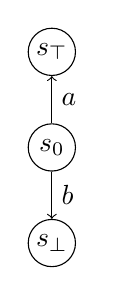
\begin{tikzpicture}	
	\node[sstate] (si) {$s_0$};
	\node[sstate,above=0.6cm of si] (s0) {$\target$};
	\node[sstate,below=0.6cm of si] (s1) {$\sink$};
	\draw[->] (si) -- node[right] {$a$} (s0);
	\draw[->] (si) -- node[right] {$b$} (s1);
	
\end{tikzpicture}
\caption{}
\end{subfigure}
\begin{subfigure}{0.38\columnwidth}
\centering
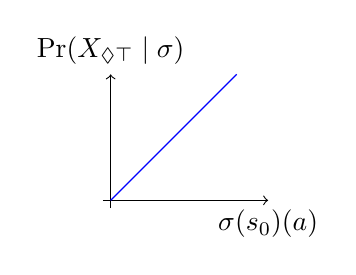
\begin{tikzpicture}[scale=2]
 \draw[->] (-0.05, 0) -- (1, 0) node[below]{$\sched(s_0)(a)$};
  	\draw[->] (0, -0.05) -- (0, 0.8) node[above] {$\Pr(X_{\lozenge\mathbf{\top}} \mid \sched)$};
  	%\draw[-,dashed] (0.4,0) -- (0.4,0.5184);
  	%\draw[-,dashed] (0.0,0.5184) -- (0.4,0.5184);
  \draw[ domain=0:0.8, smooth, variable=\x, blue] plot ({\x}, {\x});
\end{tikzpicture}
\caption{}
\end{subfigure}
\begin{subfigure}{0.38\columnwidth}
\centering
\begin{tikzpicture}[scale=2]	
 \draw[->] (-0.05, 0) -- (1, 0) node[below]{$\sched(s_0)(a)$};
  	\draw[->] (0, -0.05) -- (0, 0.8) node[above] {$H(\sched)$};
  	%\draw[-,dashed] (0.4,0) -- (0.4,0.5184);
  	%\draw[-,dashed] (0.0,0.5184) -- (0.4,0.5184);
 % \draw[ domain=0:1, smooth, variable=\x, blue] plot ({\x}, {15*(1-\x)*(1-\x)*(1-\x)*\x*\x});
\end{tikzpicture}
\caption{}
\end{subfigure}

\caption{Minimal ERCI problem.}
\end{figure}


Together, we obtain the following problem statement.
\begin{mdframed}[backgroundcolor=white!5]
\textbf{The ERCI Pareto Front Problem}:
Using the notation from the ERCI problem, find the set $\solutions \subseteq \mathbb{R}^2$.
\end{mdframed}
We are going to iteratively construct the  Pareto optimal points in $\solutions$. This yields a semi-decision procedure.
Clearly, finding $\solutions$ solves the ERCI problem, as we only need to decide whether $\langle \scthreshold, \randomness \rangle \in \solutions$.



With these facts, we are now well-equiped to develop the algorithms in Sec.~\ref{sec:mdp} for MDPs and Sec.~\ref{sec:sgs} for SGs.

Before we continue, we want to establish that Control improvisation problem is a conservative extension of deterministic case as investigated in~\cite{}.
\begin{mdframed}
\textbf{The Deterministic (Reactive) Control Improvisation (DCI) Problem~\cite{}}:
Given a \emph{deterministic} SG $\sg$, finite path sets $X_\psi$ and $X_\varphi$, and a threshold $p \in (0,1)$,  find a $\pOne$-policy $\pOneSched \in \POneScheds$  such that for every $\pTwo$-policy $\pTwoSched \in \PTwoScheds$ 
\begin{compactenum}
\item (\emph{hard constraint}) $\Pr(X_\psi \mid \sched) \geq 1$
	\item (\emph{soft constraint)} $\Pr(X_\varphi \mid \sched) \geq \scthreshold$
	\item (\emph{randomness constraint}) $\Pr(\path) \leq \delta \text{ for all } \path \in \Paths[h]{\sg[\sched]}$.
\end{compactenum}
\end{mdframed}

\begin{theorem}
	For deterministic SGs, the ERCI and DCI problem coincide.
\end{theorem}
We defer a discussion and a precise statement to Lemma~\ref{}.











\section{The Control Improvisation Problem for MDPs}
\label{sec:mdps}

We present an algorithm for the control improvisation problem for
MDPs, which in the next section, will serve as a subroutine for an
algorithm on SGs. Our goal shall be to instantiate the approximation
scheme from the previous section. In particular, we seek
to find points on the Pareto curve $\pareto{\solutions}$ and
incrementally build up $\pareto{} \subseteq \pareto{\solutions}$.
\subsection{Rationality}
To start, recall that an MDP is a stochastic game with no action
choices for the environment, i.e., the environment is purely
stochastic and the only degree of freedom is $\pOne$'s policy.  The
key idea for finding points on the Pareto-curve is to rephrase the
trade-off between randomization and performance as a degree in
rationality $\rat$ of the policy.  Formally, the rationality
corresponds to the following scalarization of our multi-objective
problem~\cite{DBLP:journals/corr/abs-1805-00909},
\begin{equation}
  \label{eq:scalarization}
  J_\rat(\sched) \eqdef \Big\langle 1, \rat\Big\rangle \cdot \Big\langle\rndp_\sched, \scp_\sched\Big\rangle.
\end{equation}
In context of MDPs, the \textbf{unique} ($\pOne$-)policy that
optimizes~\eqref{eq:scalarization} is given by a smooth variant of the
Bellman equations~\cite{mceThesis, DBLP:conf/cav/Vazquez-Chanlatte20}. Namely, let $\smoothmax{}$ denote
the log-sum-exp operator, i.e.,
$\smoothmax(X) \eqdef \log \left( \sum_{x\in X} e^x \right)$. For each
rationality $\rat \in [0, \infty)$, we define a policy $\sched_\rat$
-- using $s = \last{\path}$ -- as follows:
 \begin{align}
   &\sched_\rat(\act \mid s) \eqdef \exp( Q_\rat(s,\act) - V_\rat(s))  \label{eq:mdp:first}\\
   & V_\rat(s) \eqdef  \begin{cases}
     \lambda  \cdot \indicator{s = \target} & \text{if }s \in \{ \target, \sink \},\\
     \smoothmax_{\act \in \EnAct(s)}{  Q_\rat(s,\act) } & \text{otherwise.}
   \end{cases}\label{eq:mdp:v}\\ 
	& Q_\rat(s, \act) \eqdef \sum_{s'} P(s,\act,s') \cdot V_\rat(s').\label{eq:mdp:last}
 \end{align}
To ease notation, we denote $x_\rat \eqdef x_{\sched_\rat},
\scp_\rat \eqdef \scp_{\sched_\rat}, \rndp_\rat \eqdef
\rndp_{\sched_\rat}$. 
 % As previously alluded at the start of the subsection, the key property
% is that $\sched_\rat$ is the \emph{unique} maximum causal entropy policy
% such that $\Pr(\varphi) = \scp_\rat$~\cite{mceThesis}.
Intuitively, as $\rat \rightarrow 0$, $\sched_\rat$ approaches the
uniform distribution over \emph{all available actions}. Note that this
policy maximizes (causal) entropy, and thus $\rndopt = \rndp_0$.  As
$\lambda \rightarrow \infty$, this variant of the Bellman equations
coincides with the standard Bellman
equations~\cite{DBLP:books/wi/Puterman94}, where $\sched_\rat$ selects
(uniformly) from actions \emph{that maximize performance}.
Furthermore, the monotonicity and smoothness of the above Bellman
equations yields the following proposition.
\begin{proposition}
  $\scp_\rat$ is  continuously (and strictly) increasing in $\rat$ and $\rndp_\rat$
  is smoothly (and strictly) decreasing in $\rat$.
\end{proposition}
\noindent In terms of $\solfuncp$, we can define:
\begin{equation}
  \epsilon_\rat \eqdef \frac{\scp_\rat - \scp_0}{\scp_\infty} + \scp_0
  \hspace{1em}\text{and}\hspace{1em}
\delta_\rat \eqdef \frac{\rndp_\rat - \rndp_\infty}{\rndp_0} +
\rndp_{\infty}. 
\end{equation}

Then, because $\sched_\rat$ maximizes randomness
given a target performance, one derives:
\begin{equation}
  \solfuncp\left(\delta_\rat\right) = \epsilon_\rat.
\end{equation}

What remains is to instantiate the approximation scheme for the Pareto
front by varying the optimization direction
$\langle \rat, 1\rangle$.\footnote{Assuming $\scopt, \rndopt \neq 0$
  (which would otherwise yield trivial $\solutions$ and
  $\pareto{\solutions}$)}  In particular, we construct
$\pareto{} = \{ x_\rat \mid \rat \in \{ \rat_1, \rat_2, \hdots \} \}$
until $\pareto{}$ contains a witness to either realizability or
unrealizability of the ERCI instance. We notice that the scalarization in \eqref{eq:scalarization} means that we may additionally exploit witnesses to unrealizability as outlined in Remark~\ref{rem:scalarwitnesses}. In the remainder of this
section, we improve upon randomly selecting values for $\rat$.



%
%and by varying $\rat$ we can explore the Pareto front. First observe the following easily verified proposition.
%\begin{proposition}
%  $\scp_\rat$ is smoothly and (strictly) monotonically increasing in $\rat$ and $\rndp_\rat$
%  is smoothly (strictly) monotonically decreasing in $\rat$.
%\end{proposition}

\subsection{Targeted Pareto-exploration}
The key ingredient to improve upon arbitrarily selecting $\rat_1, \hdots \rat_i$ is to exploit additional structure of the rationality.  
%The key algorithmic idea is thus to strategically evaluate a sequence
%of rationality coefficients to yield (input, output) pairs for
%$\solfuncp$. Due to convexity, the convex hull this sequence of
%rationality-indexed points (and the origin) gradually refines a
%polygonal approximation of $\solutions$, and thus the Pareto
%Front. This approximation, $\hat{\solutions}$, is refined until
%either:
%\begin{enumerate}
%\item $\langle \scthreshold, \randomness \rangle \in \hat{\solutions}$ proving
%  $\langle \scthreshold, \randomness \rangle \in \solutions$.
%\item A $\rat$ is found such that
%  $x_{\rat} \prec \langle \scthreshold, \randomness \rangle$, proving
%  $\langle \scthreshold, \randomness \rangle \notin \solutions$.
%\end{enumerate}
%
%
%Next, to extract an improviser, observe that because
%$\hat{\solutions}$ is a convex polygon, if $\langle \scthreshold,
%\randomness \rangle \in \hat{S}$, then there must two corners of
%$\hat{\solutions}$ indexed by $\rat_1$ and $\rat_2$, that form a
%triangle with $(0, 0)$ containing $\langle \scthreshold, \randomness
%\rangle$. Thus, as in the convexity proof, there must be a convex
%combination of $q\cdot x_{\rat_1} + \bar{q}\cdot x_{\rat_2}$ that
%dominates $\langle \scthreshold, \randomness \rangle$. Therefore, the
%following policy solves the ERCI instance:

%\mypara{Approximation Sequence} 
%The final algorithmic question for
%MDPs is then: what order should one evaluate rationality coefficients.
We propose a three staged sequence: (i) Compute $x_\rat$ for the end
points $\rat \in \{0, \infty\}$.  (ii) Double $\rat$ (starting at $\lambda=1$) until $h_\rat \leq
\randomness$, yielding $\rat_1\ldots \rat_j$.
(iii) Binary search for $\rat \in [\rat_{j-1}, \rat_{j}]$. We illustrate the idea in Fig.~\ref{fig:geom:doubling}.

The algorithm terminates almost surely, that is: 
the algorithm halts if $\langle \scthreshold, \randomness \rangle$ is
not on $\pareto{\solutions}$ (or if we happen to exactly hit $\langle \scthreshold, \randomness\rangle$ by selecting some rationality $\rat$).
As the Pareto front has
measure 0, we argue that not halting is thus merely a technical concern, as a
small perturbation to the ERCI instance (i.e. a \emph{smoothed
analysis}~\cite{SmoothedAnalysis}) on $\sg$ admits decidability. 
\begin{mdframed}
  Our approximation scheme yields a semi-decision process which halts
  iff either (a) $\langle \scthreshold, \randomness \rangle$ is
  bounded away from $\pareto{\solutions}$ \emph{or} (b)
  $\langle \scthreshold, \randomness \rangle$ is dominated by
  $x_{\rat_i}$.
\end{mdframed}
Next, observe that if we terminate the binary search when the search
region is smaller than $\Delta$, this approximation scheme becomes linear in the MDP size
and logarithmic in the final rationality, $\rat_*$, and the
resolution, $\Delta$, i.e., the run-time is,
\begin{equation}
  \mathcal{O}\Big(~\hspace{-1.4em}\underbrace{|\sg|}_{\text{Evaluate $x_\rat$}}\hspace{-1.4em}~\cdot\overbrace{\log(\rat_*)}^{\text{Doubling Phase}}\cdot\underbrace{\log(\nicefrac{1}{\Delta})}_{\text{Binary Search}}\Big)
\end{equation}
Finally, before generalizing to stochastic games, we observe that in
practice, $\rat = 100$ yields a nearly optimal policy, and thus one
can often assume $\rat_* \leq 100$ in our run-time analysis.

%%% Local Variables:
%%% mode: latex
%%% TeX-master: "main"
%%% End:

 
\section{The Control Improvisation Problem for SGs}
\label{sec:sgs}
\paragraph{Maximising entropy against an adverserial player}

\subsection{Playing against deterministic adverseries}
To formalise our argument
\paragraph{Reformulation as a set of MDPs}

\paragraph{}


\subsection{Randomizing adversaries will not play better}

\subsection{Non-observable adversaries}
%\begin{mdframed}
%
%\begin{compactenum}
%	\item $\Pr^\sg_{\langle \sched_1,\sched_2 \rangle}(\eventually{h} T) \geq 1$
%	\item $\Pr^\sg_{\langle \sched_1,\sched_2 \rangle}(\eventually{h} G) \geq \lambda$ 
%\end{compactenum}
%\end{mdframed}
%\sj{Define randomly selected policy}
%\sj{Describe in terms of pMDPp}


\section{Implementation and Empirical Evaluation}
\label{sec:empirical}

\section{Discussion, Related work and Conclusion}
\label{sec:related}
\color{red}
Maybe briefly discuss synthesis algorithms mentioned at start of intro?
\color{black}

Control improvisation~\cite{DBLP:journals/corr/FremontDS17,DBLP:conf/cav/FremontS18} -- discussed in Sec.~\ref{sec:rci} -- has been used in a stochastic environment for lane changing~\cite{DBLP:conf/cdc/GeM18} and imitating power usage in households~\cite{DBLP:conf/iotdi/AkkayaFVDLS16}. However, in those both settings, the randomness constraint is phrased as an upper-bound on the probability of indefinitely-long paths. Consequently, those  randomness constraints are trivially satisfied and the obtained policies are deterministic. 
 In comparison, we consider the synthesis of policies that randomize in presence of stochastic behavior in the environment. 

Synthesis in MDPs with multiple hard and soft constraints (often over indefinite horizons) is a well-studied problem~\cite{DBLP:conf/stacs/ChatterjeeMH06,DBLP:conf/tacas/EtessamiKVY07,DBLP:conf/atva/ForejtKP12,DBLP:journals/fmsd/RandourRS17}.  In this setting, one generates deterministic policies and their convex combinations. Put differently, some degree of randomization is \emph{not an objective}, but rather a consequence. Interestingly, in \cite{DBLP:conf/tacas/DelgrangeKQR20} the optimal policies in \emph{absence} of randomization are investigated. Along similar lines, \cite{DBLP:journals/jcss/BrazdilCFK17} trades average performance for less variance, thereby implicitly trading off the average and the worst-case performance.  
The original results sparked interest in different extension to MDPs and the type of soft constraints, such as continuous MDPs \cite{DBLP:journals/csysl/HaesaertNS21} and continuous-time MDPs~\cite{DBLP:conf/cav/QuatmannJK17},  cost-bounded reachability \cite{DBLP:journals/jar/HartmannsJKQ20}, or mean-payoff properties~\cite{DBLP:journals/corr/abs-1104-3489}. 
The algorithms have also been extended towards stochastic games~\cite{DBLP:conf/mfcs/ChenFKSW13,DBLP:journals/sttt/KwiatkowskaPW18}.
Finally, notions of lexicographic multi-objective synthesis~\cite{DBLP:conf/cav/ChatterjeeKWW20} -- in which one optimizes a secondary criterion among all policies that are optimal with respect to a first criterion bare some resemblance with the algorithm we consider. 
These algorithms have been put in a robotics context in~\cite{DBLP:journals/ijrr/LacerdaFPH19}.
Finding policies that optimize reward objectives is well-studied in the field of reinforcement learning, and has been extended to generate Pareto-fronts for multiple objectives~\cite{DBLP:conf/icml/NatarajanT05,DBLP:conf/adprl/ParisiPSBR14}.

Randomization has been considered in different contexts. Entropy in MDPs is optimized in \cite{DBLP:journals/tac/SavasOCKT20}. 
\textcolor{red}{Marcell, do you have more on (causal) sentropy?}
Beyond Markov models, the (uniform) randomization over languages in finite automata \cite{DBLP:journals/siamcomp/HickeyC83,DBLP:conf/soda/KannanSM95} or over propositional formulae \cite{DBLP:journals/tcs/JerrumVV86,DBLP:journals/iandc/BellareGP00,DBLP:conf/dac/ChakrabortyMV14} has received quite some attention. Neither of those approaches support the notion of soft constraints or the related tradeoffs.

Path-finding has long been considered a multi-objective problem itself~\cite{DBLP:conf/icra/AmigoniG05,DBLP:journals/eswa/NazarahariKD19,DBLP:conf/icml/XuTMRSM20}.
These works differ prominently in two aspects: they do not trade-off randomization and performance, and they do not trade-off declarative and formal constraints with the accompanying formal guarentees, but are more search-based. 

Patrolling POIs and perimeters has received plenty of attention, e.g.,~\cite{DBLP:conf/icra/AgmonKK08,DBLP:conf/icra/AmigoniBG09,DBLP:conf/iros/PortugalPRC14}.  
Closest to our work are  formalisms rooted in game-theory,  such as  \emph{Stackelberg games}~\cite{simaan1973stackelberg,DBLP:conf/atal/ParuchuriPTOK07}. Stackelberg games have been extending to Stackelberg planning~\cite{DBLP:conf/aaai/SpeicherS00K18} in which a tradeoff between the cost for the defender and the attacker can be investigated.
Most related are the zero-sum~\emph{patrolling games} introduced in~\cite{DBLP:journals/ior/AlpernMP11}, which has led to numerous practical solutions~\cite{DBLP:books/daglib/0040483}. Patrolling games are explicitly games between an intruder and a defender, and there is no stochastic environment.  Adding additional objectives makes solving these problems harder~\cite{DBLP:conf/atal/Klaska0R20} and in general, the obtained policies are no longer applicable. To overcome this, a specific set of fixed objectives has been added to these games recently~\cite{DBLP:conf/atal/Klaska0R20}. 
 The large common aspect in all of this work is that optimal strategies do randomize. As in the synthesis work above, this is a consequence of the objectives rather than an objective in itself. 
In comparison, we provide a general framework and in particular support stochastic environments.
\bibliographystyle{plainnat}
\bibliography{bibliography}

\end{document}
